\subsection{Basic Distance}

In order to have a template and a point of comparison for our following work, we started with a simple and intuitive metric.

\subsubsection{The formula}

The distance calculation is based on the common words between two subsets $C_1$ and $C_2$ of the corpus. The distance $d(C_1,C_2)$ is defined as follows:
\begin{eqnarray}
 d(C_1,C_2) = 1 - \frac{2 \Arrowvert C_1 \cap C_2\Arrowvert}{\Arrowvert C_1 \Arrowvert + \Arrowvert C_2 \Arrowvert }
\end{eqnarray}
where $\Arrowvert \cdot \Arrowvert$ denotes here the number of distinct words and $C_1 \cap C_2$ is the set containing the common words between $C_1$ and $C_2$.

\subsubsection{Computations on the corpus}

We applied the basic distance on the years contained in the corrected corpus, producing the following matrix:

\begin{figure}[H]
    \centering
    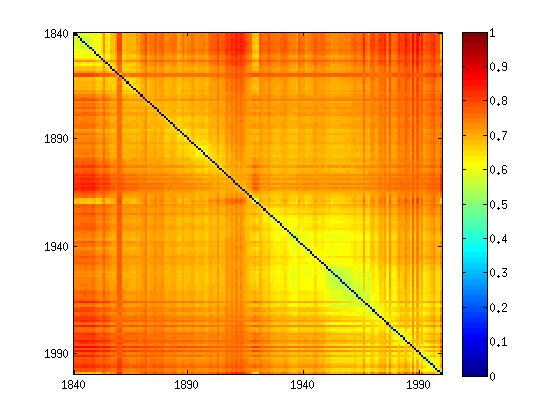
\includegraphics[scale=0.4]{Pictures/distance1/d1.jpg}
    \caption{Basic distance for 1-gram with OCR correction}
    \label{D1}
\end{figure}

\subsubsection{Analysis}

As our goal is to find a metric that can show a linguistic drift, consecutive years should have a distance near zero and distant years should have a distance close to one. In figure \ref{D1}, if we take for example the year 1940, the distance with itself is zero as wanted. But the distance with 1939 or 1941 is jumping over 0.5. Those kind of jumps around the zero diagonal are the behaviour we want to avoid and this distance is definitely not good.